\chapter{Chorale harmonization}\label{ch:harmonization}

% **************************** Define Graphics Path **************************
\ifpdf
    \graphicspath{{Chapter6/Figs/Raster/}{Chapter6/Figs/PDF/}{Chapter6/Figs/}}
\else
    \graphicspath{{Chapter6/Figs/Vector/}{Chapter6/Figs/}}
\fi

Every aspiring music theorist is at some point tasked with composing simple
pieces of music in order demonstrate understanding of the harmonic rules of
Western classical music. These pedagogical exercises often include
harmonization of chorale melodies, a task which is viewed as sufficiently
constrained to allow a composer's basic technique to be judged.

Mirroring the pedagogy for music students, this chapter evaluates the learned
deep LSTM model's ability on various harmonization tasks. Unlike automatic
composition, where the model is free compose a score of music without any
constraints, in harmonization tasks one or more of the parts are fixed and only
the remaining are generated.

In music education, harmonization of a given melody is considered a more
elementary task than generation of a novel chorale
\citep{denny1960oxford,piston1978harmony}. However, these expectations may not
be valid for our model, which was trained without any consideration of the
future notes occurring in the provided melody. Our experiments in this chapter
will yield a definitive answer to this question.

% \section{Introduction to chorale harmonization}

% as described by Walter Piston \citep{piston1978harmony}:

% \begin{quote}
%   True harmonisation, then, means a consideration of the alternatives in
%   available chords, the reasoned selection of one of these alternatives, and
%   the tasteful arrangement of the texture of the added parts with due regard
%   for consistency of style
% \end{quote}

% The Baroque style employed by Bach has specific guidelines
% such as disallowing parallel fifths and parallel octaves as well as
% considerations for voice leading \citep{piston1978harmony}.

% For a music student studying chorale harmonization, a common pedagogical
% exercise \citep{denny1960oxford}\citep{piston1978harmony} is a sequence of tasks increasing in difficulty:
% \begin{enumerate}
%   \item Providing either alto or tenor given fixed soprano and bass
%   \item Providing both alto and tenor parts given fixed soprano and bass
%   \item Harmonization: provide all remaining parts given only the soprano line
%   \item Composition: provide all four parts with nothing given in advance
% \end{enumerate}

% There are no definitive formalization of the harmonization process, making
% evaluation difficult. Attenpts to formalize the process using Shenkerian
% structural analysis \citep{schenker1954harmony} and symbolic methods such as
% generative grammars \citep{lerdahl1983jackendoff}\citep{winograd1968linguistics}
% exist, but involve human analytical process.

\section{Adapting the automatic composition model}

\nomenclature[a-Pstar]{$P^*$}{true probability distribution}
\nomenclature[a-Ptilde]{$\tilde{P}$}{distribution predicted by model}
\nomenclature[a-xstar]{$\x^*$}{the optimal harmonization}
\nomenclature[a-xtilde]{$\tilde{\x}$}{the proposed harmonization}
\nomenclature[a-xhat]{$\hat{\x}$}{values of fixed tokens in a harmonization}
\nomenclature[g-alpha]{$\alpha$}{multi-index of fixed tokens in harmonization}
\nomenclature[g-delta]{$\delta$}{Kroneker delta}

Recall that \cref{ch:model-analysis} gave us a RNN model
$\tilde{P}(\vec{x}_{t+1} | \vec{x}_{t}, \h_{t-1})$, which combined with a fixed
initial hidden state $\h_0$ yields a \emph{sequential prediction model}
$\tilde{P}(\x_t | \x_{1:t-1})$ approximating the \emph{true distribution}
$P^*(\x_{t+1} | \x_{t})$. In this section, we describe a method for applying
such a sequential prediction model to produce chorale harmonizations. The
proposed technique is equivalent to a $1$-best greedy search through a lattice
constrained by the fixed melody line, and we will explore how solutions from
the lattice processing literature might be applied.

In chorale harmonization, we are tasked to compose the notes for a subset of
parts which are harmonically and stylistically compatible with the fixed parts.
To be concrete, let $\{\x_{t}\}_{t=1}^T$ be a \emph{sequence of tokens}
representing an encoded score. Let $\alpha \subset \{1,2,\cdots,T\}$ be \emph{a
multi-index} and suppose $\hat{\x}_{\alpha}$ correspond to the \emph{fixed
token values for the given parts} in the harmonization task. We are interested
in optimizing the conditional distribution:
\begin{equation}
  \x_{1:T}^* = \argmax_{x_{1:L}} P(\x_{1:L} | \x_{\alpha} = \hat{\x}_\alpha )
\end{equation}
First, any \emph{proposed solution} $\tilde{\x}_{1:T}$ must satisfy
$\tilde{\x}_{\alpha} = \hat{\x}_\alpha$, so the only decision variables are
$\tilde{\x}_{\alpha^c}$ where $\alpha^c \coloneqq \{1,2,\cdots,T\} \setminus
\alpha$. \citet{hinton1986learning} refer to this constraint as ``clamping''
the generative model.

The remaining task is to choose values for $\tilde{\x}_{\alpha^c}$.
We propose a simple greedy strategy:
\begin{equation}\label{eq:greedy-harmonization}
  \tilde{\x}_{t} = \begin{cases}
    \hat{\x}_{t} &\text{if}~t \in \alpha \\
    \argmax_{\x_t} P(\x_t | \tilde{\x}_{1:t-1}) &\text{otherwise}
  \end{cases}
\end{equation}
where the tilde on the previous tokens $\tilde{\x}_{1:t-1}$ indicate that they are
equal to the actual previous $\argmax$ choices.

\subsection{Shortcomings of the proposed model}\label{sec:shortcomings-harm}

We admit that this approach is a greedy approximation: we are not guaranteed
$\hat{\x}_{1:T}$. In fact, we can view the problem as a search over a lattice
of possible trajectories $\tilde{\x}_{1:T}$ constrained such that
$\tilde{\x}_{\alpha} = \hat{\x}_\alpha$. Under the lattice framework, our
strategy is recognized as a beam search with beam width $1$. A wider beam-width
which maintained $N$-best hypotheses such as in \citet{liu2014efficient} would
allow the model to partially recover from mistakes made by greedy action
selection. We leave this extension for future work.

% We make the 
% \begin{itemize}
%   \item Modeling capacity limits for RNNs: the model $\hat{P}$ may not be able to fully express
%     the true distribution $P$ (\eg if $P$ is non-Markovian)
%   \item Greedy sequential selection: it is possible that the greedy $\argmax$ at each
%     time without accounting for future constraints on sequences $(w_{\alpha_{t'}})_{t' > t}$
%     leads to a solution with sub-optimal joint probability
%   \item Assumption that prior selections $\hat{w_{1:t-1}}$ optimize $P(w_t | w_{1:t-1})$:
%     the model $\hat{P}$ is trained on data which assumes all prior inputs have beeen
%     ground truth. It has been shown \mynote{mikolov} that such an assumption can lead to
%     very sensitive hidden state dynamics which are not robust to errors (\ie when
%     $\hat{w_{1:t-1}}$ contain errors).
% \end{itemize}
% Beam search is one way to mitigate the effects of greedy selection: our current
% method is equivalent to a beam search with width one. Maintaining $N$-best
% hypotheses using a lattice-based framework such as in \citet{liu2014efficient}
% would 

% Another potential issue with the proposed model is a discrepancy between the
% inputs provided during training (which are taken from actual data sequences
% regargless of model predictions) and sampling (where the inputs are generated
% by the model at the previous timestep). To resolve this discrepancy,
% \citet{bengio2015scheduled} proposed \emph{scheduled sampling} as a curriculum
% learning strategy gradually transitioning sequence models to rely on their
% prior predictions as inputs and thereby learn state dynamics more resilient to
% erroneous inputs.

% Despite these limitations, implementation of greedy action selection is still
% valuable because it forms the basis for more sophisticated lattice-based search
% methods as well as provides a baseline for comparing performance against.

\section{Datasets}\label{sec:harm-dataset}

\nomenclature[z-S]{S}{Soprano}
\nomenclature[z-A]{A}{Alto}
\nomenclature[z-T]{T}{Tenor}
\nomenclature[z-B]{B}{Bass}
\nomenclature[z-AT]{AT}{Alto and Tenor}
\nomenclature[z-ATB]{ATB}{Alto, Tenor, and Bass}
\nomenclature[z-SATB]{SATB}{Soprano, Alto, Tenor, and Bass}

We create datasets where one or more parts are to be harmonized by the model:
\begin{enumerate}
  \item A single parts: Soprano (S), Alto (A), Tenor (T), or Bass (B).
  \item The middle two parts (AT).
  \item All parts except Soprano (ATB). This is what is usually meant by \emph{harmonization}.
\end{enumerate}
It is widely accepted that these tasks successively increase in terms of
difficulty \citep{denny1960oxford}. Of particular interest is the AT case.
Bach oftentimes only wrote the Soprano and Bass parts of a piece, leaving the
middle parts to be filled in by students. Based on these observations, we
hypothesize that performance will be similar for harmonizing any single part
and successively deteriorate for the AT and ATB cases respectively.

\section{Results}
\label{sec:harmonization-results}

\nomenclature[z-ter]{TER}{Token Error Rate}
\nomenclature[z-fer]{FER}{Frame Error Rate}

\subsection{Error rates harmonizing Bach chorales}

We deleted different subsets of parts from a held-out validation corpus
consisting of $10\%$ of the data and used the method proposed in
\cref{eq:greedy-harmonization} to harmonize the missing parts. We evaluate
our model's error rate predicting individual tokens (\emph{token error rate}, TER)
as well as all tokens within frames (\emph{frame error rate}, FER) and show
our results in \cref{fig:harmonization-results}.

\begin{figure}[tb]
  \centering
  %% Creator: Matplotlib, PGF backend
%%
%% To include the figure in your LaTeX document, write
%%   \input{<filename>.pgf}
%%
%% Make sure the required packages are loaded in your preamble
%%   \usepackage{pgf}
%%
%% Figures using additional raster images can only be included by \input if
%% they are in the same directory as the main LaTeX file. For loading figures
%% from other directories you can use the `import` package
%%   \usepackage{import}
%% and then include the figures with
%%   \import{<path to file>}{<filename>.pgf}
%%
%% Matplotlib used the following preamble
%%   \usepackage[utf8x]{inputenc}
%%   \usepackage[T1]{fontenc}
%%   \usepackage{fontspec}
%%
\begingroup%
\makeatletter%
\begin{pgfpicture}%
\pgfpathrectangle{\pgfpointorigin}{\pgfqpoint{4.608901in}{2.829111in}}%
\pgfusepath{use as bounding box, clip}%
\begin{pgfscope}%
\pgfsetbuttcap%
\pgfsetmiterjoin%
\definecolor{currentfill}{rgb}{1.000000,1.000000,1.000000}%
\pgfsetfillcolor{currentfill}%
\pgfsetlinewidth{0.000000pt}%
\definecolor{currentstroke}{rgb}{1.000000,1.000000,1.000000}%
\pgfsetstrokecolor{currentstroke}%
\pgfsetdash{}{0pt}%
\pgfpathmoveto{\pgfqpoint{0.000000in}{-0.000000in}}%
\pgfpathlineto{\pgfqpoint{4.608901in}{-0.000000in}}%
\pgfpathlineto{\pgfqpoint{4.608901in}{2.829111in}}%
\pgfpathlineto{\pgfqpoint{0.000000in}{2.829111in}}%
\pgfpathclose%
\pgfusepath{fill}%
\end{pgfscope}%
\begin{pgfscope}%
\pgfsetbuttcap%
\pgfsetmiterjoin%
\definecolor{currentfill}{rgb}{0.917647,0.917647,0.949020}%
\pgfsetfillcolor{currentfill}%
\pgfsetlinewidth{0.000000pt}%
\definecolor{currentstroke}{rgb}{0.000000,0.000000,0.000000}%
\pgfsetstrokecolor{currentstroke}%
\pgfsetstrokeopacity{0.000000}%
\pgfsetdash{}{0pt}%
\pgfpathmoveto{\pgfqpoint{0.540851in}{0.605814in}}%
\pgfpathlineto{\pgfqpoint{3.800901in}{0.605814in}}%
\pgfpathlineto{\pgfqpoint{3.800901in}{2.544000in}}%
\pgfpathlineto{\pgfqpoint{0.540851in}{2.544000in}}%
\pgfpathclose%
\pgfusepath{fill}%
\end{pgfscope}%
\begin{pgfscope}%
\pgfsetbuttcap%
\pgfsetmiterjoin%
\definecolor{currentfill}{rgb}{1.000000,1.000000,1.000000}%
\pgfsetfillcolor{currentfill}%
\pgfsetlinewidth{0.301125pt}%
\definecolor{currentstroke}{rgb}{0.000000,0.000000,0.000000}%
\pgfsetstrokecolor{currentstroke}%
\pgfsetdash{}{0pt}%
\pgfpathmoveto{\pgfqpoint{0.540851in}{0.437210in}}%
\pgfpathlineto{\pgfqpoint{1.084193in}{0.437210in}}%
\pgfpathlineto{\pgfqpoint{1.084193in}{0.605814in}}%
\pgfpathlineto{\pgfqpoint{0.540851in}{0.605814in}}%
\pgfpathclose%
\pgfusepath{stroke,fill}%
\end{pgfscope}%
\begin{pgfscope}%
\definecolor{textcolor}{rgb}{0.150000,0.150000,0.150000}%
\pgfsetstrokecolor{textcolor}%
\pgfsetfillcolor{textcolor}%
\pgftext[x=0.812522in,y=0.521512in,,]{\color{textcolor}\rmfamily\fontsize{10.000000}{12.000000}\selectfont S}%
\end{pgfscope}%
\begin{pgfscope}%
\pgfsetbuttcap%
\pgfsetmiterjoin%
\definecolor{currentfill}{rgb}{1.000000,1.000000,1.000000}%
\pgfsetfillcolor{currentfill}%
\pgfsetlinewidth{0.301125pt}%
\definecolor{currentstroke}{rgb}{0.000000,0.000000,0.000000}%
\pgfsetstrokecolor{currentstroke}%
\pgfsetdash{}{0pt}%
\pgfpathmoveto{\pgfqpoint{1.084193in}{0.437210in}}%
\pgfpathlineto{\pgfqpoint{1.627534in}{0.437210in}}%
\pgfpathlineto{\pgfqpoint{1.627534in}{0.605814in}}%
\pgfpathlineto{\pgfqpoint{1.084193in}{0.605814in}}%
\pgfpathclose%
\pgfusepath{stroke,fill}%
\end{pgfscope}%
\begin{pgfscope}%
\definecolor{textcolor}{rgb}{0.150000,0.150000,0.150000}%
\pgfsetstrokecolor{textcolor}%
\pgfsetfillcolor{textcolor}%
\pgftext[x=1.355863in,y=0.521512in,,]{\color{textcolor}\rmfamily\fontsize{10.000000}{12.000000}\selectfont A}%
\end{pgfscope}%
\begin{pgfscope}%
\pgfsetbuttcap%
\pgfsetmiterjoin%
\definecolor{currentfill}{rgb}{1.000000,1.000000,1.000000}%
\pgfsetfillcolor{currentfill}%
\pgfsetlinewidth{0.301125pt}%
\definecolor{currentstroke}{rgb}{0.000000,0.000000,0.000000}%
\pgfsetstrokecolor{currentstroke}%
\pgfsetdash{}{0pt}%
\pgfpathmoveto{\pgfqpoint{1.627534in}{0.437210in}}%
\pgfpathlineto{\pgfqpoint{2.170876in}{0.437210in}}%
\pgfpathlineto{\pgfqpoint{2.170876in}{0.605814in}}%
\pgfpathlineto{\pgfqpoint{1.627534in}{0.605814in}}%
\pgfpathclose%
\pgfusepath{stroke,fill}%
\end{pgfscope}%
\begin{pgfscope}%
\definecolor{textcolor}{rgb}{0.150000,0.150000,0.150000}%
\pgfsetstrokecolor{textcolor}%
\pgfsetfillcolor{textcolor}%
\pgftext[x=1.899205in,y=0.521512in,,]{\color{textcolor}\rmfamily\fontsize{10.000000}{12.000000}\selectfont T}%
\end{pgfscope}%
\begin{pgfscope}%
\pgfsetbuttcap%
\pgfsetmiterjoin%
\definecolor{currentfill}{rgb}{1.000000,1.000000,1.000000}%
\pgfsetfillcolor{currentfill}%
\pgfsetlinewidth{0.301125pt}%
\definecolor{currentstroke}{rgb}{0.000000,0.000000,0.000000}%
\pgfsetstrokecolor{currentstroke}%
\pgfsetdash{}{0pt}%
\pgfpathmoveto{\pgfqpoint{2.170876in}{0.437210in}}%
\pgfpathlineto{\pgfqpoint{2.714218in}{0.437210in}}%
\pgfpathlineto{\pgfqpoint{2.714218in}{0.605814in}}%
\pgfpathlineto{\pgfqpoint{2.170876in}{0.605814in}}%
\pgfpathclose%
\pgfusepath{stroke,fill}%
\end{pgfscope}%
\begin{pgfscope}%
\definecolor{textcolor}{rgb}{0.150000,0.150000,0.150000}%
\pgfsetstrokecolor{textcolor}%
\pgfsetfillcolor{textcolor}%
\pgftext[x=2.442547in,y=0.521512in,,]{\color{textcolor}\rmfamily\fontsize{10.000000}{12.000000}\selectfont B}%
\end{pgfscope}%
\begin{pgfscope}%
\pgfsetbuttcap%
\pgfsetmiterjoin%
\definecolor{currentfill}{rgb}{1.000000,1.000000,1.000000}%
\pgfsetfillcolor{currentfill}%
\pgfsetlinewidth{0.301125pt}%
\definecolor{currentstroke}{rgb}{0.000000,0.000000,0.000000}%
\pgfsetstrokecolor{currentstroke}%
\pgfsetdash{}{0pt}%
\pgfpathmoveto{\pgfqpoint{2.714218in}{0.437210in}}%
\pgfpathlineto{\pgfqpoint{3.257560in}{0.437210in}}%
\pgfpathlineto{\pgfqpoint{3.257560in}{0.605814in}}%
\pgfpathlineto{\pgfqpoint{2.714218in}{0.605814in}}%
\pgfpathclose%
\pgfusepath{stroke,fill}%
\end{pgfscope}%
\begin{pgfscope}%
\definecolor{textcolor}{rgb}{0.150000,0.150000,0.150000}%
\pgfsetstrokecolor{textcolor}%
\pgfsetfillcolor{textcolor}%
\pgftext[x=2.985889in,y=0.521512in,,]{\color{textcolor}\rmfamily\fontsize{10.000000}{12.000000}\selectfont AT}%
\end{pgfscope}%
\begin{pgfscope}%
\pgfsetbuttcap%
\pgfsetmiterjoin%
\definecolor{currentfill}{rgb}{1.000000,1.000000,1.000000}%
\pgfsetfillcolor{currentfill}%
\pgfsetlinewidth{0.301125pt}%
\definecolor{currentstroke}{rgb}{0.000000,0.000000,0.000000}%
\pgfsetstrokecolor{currentstroke}%
\pgfsetdash{}{0pt}%
\pgfpathmoveto{\pgfqpoint{3.257560in}{0.437210in}}%
\pgfpathlineto{\pgfqpoint{3.800901in}{0.437210in}}%
\pgfpathlineto{\pgfqpoint{3.800901in}{0.605814in}}%
\pgfpathlineto{\pgfqpoint{3.257560in}{0.605814in}}%
\pgfpathclose%
\pgfusepath{stroke,fill}%
\end{pgfscope}%
\begin{pgfscope}%
\definecolor{textcolor}{rgb}{0.150000,0.150000,0.150000}%
\pgfsetstrokecolor{textcolor}%
\pgfsetfillcolor{textcolor}%
\pgftext[x=3.529230in,y=0.521512in,,]{\color{textcolor}\rmfamily\fontsize{10.000000}{12.000000}\selectfont ATB}%
\end{pgfscope}%
\begin{pgfscope}%
\pgfsetbuttcap%
\pgfsetmiterjoin%
\definecolor{currentfill}{rgb}{1.000000,1.000000,1.000000}%
\pgfsetfillcolor{currentfill}%
\pgfsetlinewidth{0.301125pt}%
\definecolor{currentstroke}{rgb}{0.000000,0.000000,0.000000}%
\pgfsetstrokecolor{currentstroke}%
\pgfsetdash{}{0pt}%
\pgfpathmoveto{\pgfqpoint{0.184351in}{0.268605in}}%
\pgfpathlineto{\pgfqpoint{0.540851in}{0.268605in}}%
\pgfpathlineto{\pgfqpoint{0.540851in}{0.437210in}}%
\pgfpathlineto{\pgfqpoint{0.184351in}{0.437210in}}%
\pgfpathclose%
\pgfusepath{stroke,fill}%
\end{pgfscope}%
\begin{pgfscope}%
\definecolor{textcolor}{rgb}{0.150000,0.150000,0.150000}%
\pgfsetstrokecolor{textcolor}%
\pgfsetfillcolor{textcolor}%
\pgftext[x=0.220001in,y=0.352907in,left,]{\color{textcolor}\rmfamily\fontsize{10.000000}{12.000000}\selectfont TER}%
\end{pgfscope}%
\begin{pgfscope}%
\pgfsetbuttcap%
\pgfsetmiterjoin%
\definecolor{currentfill}{rgb}{1.000000,1.000000,1.000000}%
\pgfsetfillcolor{currentfill}%
\pgfsetlinewidth{0.301125pt}%
\definecolor{currentstroke}{rgb}{0.000000,0.000000,0.000000}%
\pgfsetstrokecolor{currentstroke}%
\pgfsetdash{}{0pt}%
\pgfpathmoveto{\pgfqpoint{0.540851in}{0.268605in}}%
\pgfpathlineto{\pgfqpoint{1.084193in}{0.268605in}}%
\pgfpathlineto{\pgfqpoint{1.084193in}{0.437210in}}%
\pgfpathlineto{\pgfqpoint{0.540851in}{0.437210in}}%
\pgfpathclose%
\pgfusepath{stroke,fill}%
\end{pgfscope}%
\begin{pgfscope}%
\definecolor{textcolor}{rgb}{0.150000,0.150000,0.150000}%
\pgfsetstrokecolor{textcolor}%
\pgfsetfillcolor{textcolor}%
\pgftext[x=1.029858in,y=0.352907in,right,]{\color{textcolor}\rmfamily\fontsize{10.000000}{12.000000}\selectfont 0.532}%
\end{pgfscope}%
\begin{pgfscope}%
\pgfsetbuttcap%
\pgfsetmiterjoin%
\definecolor{currentfill}{rgb}{1.000000,1.000000,1.000000}%
\pgfsetfillcolor{currentfill}%
\pgfsetlinewidth{0.301125pt}%
\definecolor{currentstroke}{rgb}{0.000000,0.000000,0.000000}%
\pgfsetstrokecolor{currentstroke}%
\pgfsetdash{}{0pt}%
\pgfpathmoveto{\pgfqpoint{1.084193in}{0.268605in}}%
\pgfpathlineto{\pgfqpoint{1.627534in}{0.268605in}}%
\pgfpathlineto{\pgfqpoint{1.627534in}{0.437210in}}%
\pgfpathlineto{\pgfqpoint{1.084193in}{0.437210in}}%
\pgfpathclose%
\pgfusepath{stroke,fill}%
\end{pgfscope}%
\begin{pgfscope}%
\definecolor{textcolor}{rgb}{0.150000,0.150000,0.150000}%
\pgfsetstrokecolor{textcolor}%
\pgfsetfillcolor{textcolor}%
\pgftext[x=1.573200in,y=0.352907in,right,]{\color{textcolor}\rmfamily\fontsize{10.000000}{12.000000}\selectfont 0.442}%
\end{pgfscope}%
\begin{pgfscope}%
\pgfsetbuttcap%
\pgfsetmiterjoin%
\definecolor{currentfill}{rgb}{1.000000,1.000000,1.000000}%
\pgfsetfillcolor{currentfill}%
\pgfsetlinewidth{0.301125pt}%
\definecolor{currentstroke}{rgb}{0.000000,0.000000,0.000000}%
\pgfsetstrokecolor{currentstroke}%
\pgfsetdash{}{0pt}%
\pgfpathmoveto{\pgfqpoint{1.627534in}{0.268605in}}%
\pgfpathlineto{\pgfqpoint{2.170876in}{0.268605in}}%
\pgfpathlineto{\pgfqpoint{2.170876in}{0.437210in}}%
\pgfpathlineto{\pgfqpoint{1.627534in}{0.437210in}}%
\pgfpathclose%
\pgfusepath{stroke,fill}%
\end{pgfscope}%
\begin{pgfscope}%
\definecolor{textcolor}{rgb}{0.150000,0.150000,0.150000}%
\pgfsetstrokecolor{textcolor}%
\pgfsetfillcolor{textcolor}%
\pgftext[x=2.116542in,y=0.352907in,right,]{\color{textcolor}\rmfamily\fontsize{10.000000}{12.000000}\selectfont 0.235}%
\end{pgfscope}%
\begin{pgfscope}%
\pgfsetbuttcap%
\pgfsetmiterjoin%
\definecolor{currentfill}{rgb}{1.000000,1.000000,1.000000}%
\pgfsetfillcolor{currentfill}%
\pgfsetlinewidth{0.301125pt}%
\definecolor{currentstroke}{rgb}{0.000000,0.000000,0.000000}%
\pgfsetstrokecolor{currentstroke}%
\pgfsetdash{}{0pt}%
\pgfpathmoveto{\pgfqpoint{2.170876in}{0.268605in}}%
\pgfpathlineto{\pgfqpoint{2.714218in}{0.268605in}}%
\pgfpathlineto{\pgfqpoint{2.714218in}{0.437210in}}%
\pgfpathlineto{\pgfqpoint{2.170876in}{0.437210in}}%
\pgfpathclose%
\pgfusepath{stroke,fill}%
\end{pgfscope}%
\begin{pgfscope}%
\definecolor{textcolor}{rgb}{0.150000,0.150000,0.150000}%
\pgfsetstrokecolor{textcolor}%
\pgfsetfillcolor{textcolor}%
\pgftext[x=2.659884in,y=0.352907in,right,]{\color{textcolor}\rmfamily\fontsize{10.000000}{12.000000}\selectfont 0.241}%
\end{pgfscope}%
\begin{pgfscope}%
\pgfsetbuttcap%
\pgfsetmiterjoin%
\definecolor{currentfill}{rgb}{1.000000,1.000000,1.000000}%
\pgfsetfillcolor{currentfill}%
\pgfsetlinewidth{0.301125pt}%
\definecolor{currentstroke}{rgb}{0.000000,0.000000,0.000000}%
\pgfsetstrokecolor{currentstroke}%
\pgfsetdash{}{0pt}%
\pgfpathmoveto{\pgfqpoint{2.714218in}{0.268605in}}%
\pgfpathlineto{\pgfqpoint{3.257560in}{0.268605in}}%
\pgfpathlineto{\pgfqpoint{3.257560in}{0.437210in}}%
\pgfpathlineto{\pgfqpoint{2.714218in}{0.437210in}}%
\pgfpathclose%
\pgfusepath{stroke,fill}%
\end{pgfscope}%
\begin{pgfscope}%
\definecolor{textcolor}{rgb}{0.150000,0.150000,0.150000}%
\pgfsetstrokecolor{textcolor}%
\pgfsetfillcolor{textcolor}%
\pgftext[x=3.203225in,y=0.352907in,right,]{\color{textcolor}\rmfamily\fontsize{10.000000}{12.000000}\selectfont 0.686}%
\end{pgfscope}%
\begin{pgfscope}%
\pgfsetbuttcap%
\pgfsetmiterjoin%
\definecolor{currentfill}{rgb}{1.000000,1.000000,1.000000}%
\pgfsetfillcolor{currentfill}%
\pgfsetlinewidth{0.301125pt}%
\definecolor{currentstroke}{rgb}{0.000000,0.000000,0.000000}%
\pgfsetstrokecolor{currentstroke}%
\pgfsetdash{}{0pt}%
\pgfpathmoveto{\pgfqpoint{3.257560in}{0.268605in}}%
\pgfpathlineto{\pgfqpoint{3.800901in}{0.268605in}}%
\pgfpathlineto{\pgfqpoint{3.800901in}{0.437210in}}%
\pgfpathlineto{\pgfqpoint{3.257560in}{0.437210in}}%
\pgfpathclose%
\pgfusepath{stroke,fill}%
\end{pgfscope}%
\begin{pgfscope}%
\definecolor{textcolor}{rgb}{0.150000,0.150000,0.150000}%
\pgfsetstrokecolor{textcolor}%
\pgfsetfillcolor{textcolor}%
\pgftext[x=3.746567in,y=0.352907in,right,]{\color{textcolor}\rmfamily\fontsize{10.000000}{12.000000}\selectfont 0.718}%
\end{pgfscope}%
\begin{pgfscope}%
\pgfsetbuttcap%
\pgfsetmiterjoin%
\definecolor{currentfill}{rgb}{1.000000,1.000000,1.000000}%
\pgfsetfillcolor{currentfill}%
\pgfsetlinewidth{0.301125pt}%
\definecolor{currentstroke}{rgb}{0.000000,0.000000,0.000000}%
\pgfsetstrokecolor{currentstroke}%
\pgfsetdash{}{0pt}%
\pgfpathmoveto{\pgfqpoint{0.184351in}{0.100000in}}%
\pgfpathlineto{\pgfqpoint{0.540851in}{0.100000in}}%
\pgfpathlineto{\pgfqpoint{0.540851in}{0.268605in}}%
\pgfpathlineto{\pgfqpoint{0.184351in}{0.268605in}}%
\pgfpathclose%
\pgfusepath{stroke,fill}%
\end{pgfscope}%
\begin{pgfscope}%
\definecolor{textcolor}{rgb}{0.150000,0.150000,0.150000}%
\pgfsetstrokecolor{textcolor}%
\pgfsetfillcolor{textcolor}%
\pgftext[x=0.220001in,y=0.184302in,left,]{\color{textcolor}\rmfamily\fontsize{10.000000}{12.000000}\selectfont FER}%
\end{pgfscope}%
\begin{pgfscope}%
\pgfsetbuttcap%
\pgfsetmiterjoin%
\definecolor{currentfill}{rgb}{1.000000,1.000000,1.000000}%
\pgfsetfillcolor{currentfill}%
\pgfsetlinewidth{0.301125pt}%
\definecolor{currentstroke}{rgb}{0.000000,0.000000,0.000000}%
\pgfsetstrokecolor{currentstroke}%
\pgfsetdash{}{0pt}%
\pgfpathmoveto{\pgfqpoint{0.540851in}{0.100000in}}%
\pgfpathlineto{\pgfqpoint{1.084193in}{0.100000in}}%
\pgfpathlineto{\pgfqpoint{1.084193in}{0.268605in}}%
\pgfpathlineto{\pgfqpoint{0.540851in}{0.268605in}}%
\pgfpathclose%
\pgfusepath{stroke,fill}%
\end{pgfscope}%
\begin{pgfscope}%
\definecolor{textcolor}{rgb}{0.150000,0.150000,0.150000}%
\pgfsetstrokecolor{textcolor}%
\pgfsetfillcolor{textcolor}%
\pgftext[x=1.029858in,y=0.184302in,right,]{\color{textcolor}\rmfamily\fontsize{10.000000}{12.000000}\selectfont 0.532}%
\end{pgfscope}%
\begin{pgfscope}%
\pgfsetbuttcap%
\pgfsetmiterjoin%
\definecolor{currentfill}{rgb}{1.000000,1.000000,1.000000}%
\pgfsetfillcolor{currentfill}%
\pgfsetlinewidth{0.301125pt}%
\definecolor{currentstroke}{rgb}{0.000000,0.000000,0.000000}%
\pgfsetstrokecolor{currentstroke}%
\pgfsetdash{}{0pt}%
\pgfpathmoveto{\pgfqpoint{1.084193in}{0.100000in}}%
\pgfpathlineto{\pgfqpoint{1.627534in}{0.100000in}}%
\pgfpathlineto{\pgfqpoint{1.627534in}{0.268605in}}%
\pgfpathlineto{\pgfqpoint{1.084193in}{0.268605in}}%
\pgfpathclose%
\pgfusepath{stroke,fill}%
\end{pgfscope}%
\begin{pgfscope}%
\definecolor{textcolor}{rgb}{0.150000,0.150000,0.150000}%
\pgfsetstrokecolor{textcolor}%
\pgfsetfillcolor{textcolor}%
\pgftext[x=1.573200in,y=0.184302in,right,]{\color{textcolor}\rmfamily\fontsize{10.000000}{12.000000}\selectfont 0.442}%
\end{pgfscope}%
\begin{pgfscope}%
\pgfsetbuttcap%
\pgfsetmiterjoin%
\definecolor{currentfill}{rgb}{1.000000,1.000000,1.000000}%
\pgfsetfillcolor{currentfill}%
\pgfsetlinewidth{0.301125pt}%
\definecolor{currentstroke}{rgb}{0.000000,0.000000,0.000000}%
\pgfsetstrokecolor{currentstroke}%
\pgfsetdash{}{0pt}%
\pgfpathmoveto{\pgfqpoint{1.627534in}{0.100000in}}%
\pgfpathlineto{\pgfqpoint{2.170876in}{0.100000in}}%
\pgfpathlineto{\pgfqpoint{2.170876in}{0.268605in}}%
\pgfpathlineto{\pgfqpoint{1.627534in}{0.268605in}}%
\pgfpathclose%
\pgfusepath{stroke,fill}%
\end{pgfscope}%
\begin{pgfscope}%
\definecolor{textcolor}{rgb}{0.150000,0.150000,0.150000}%
\pgfsetstrokecolor{textcolor}%
\pgfsetfillcolor{textcolor}%
\pgftext[x=2.116542in,y=0.184302in,right,]{\color{textcolor}\rmfamily\fontsize{10.000000}{12.000000}\selectfont 0.235}%
\end{pgfscope}%
\begin{pgfscope}%
\pgfsetbuttcap%
\pgfsetmiterjoin%
\definecolor{currentfill}{rgb}{1.000000,1.000000,1.000000}%
\pgfsetfillcolor{currentfill}%
\pgfsetlinewidth{0.301125pt}%
\definecolor{currentstroke}{rgb}{0.000000,0.000000,0.000000}%
\pgfsetstrokecolor{currentstroke}%
\pgfsetdash{}{0pt}%
\pgfpathmoveto{\pgfqpoint{2.170876in}{0.100000in}}%
\pgfpathlineto{\pgfqpoint{2.714218in}{0.100000in}}%
\pgfpathlineto{\pgfqpoint{2.714218in}{0.268605in}}%
\pgfpathlineto{\pgfqpoint{2.170876in}{0.268605in}}%
\pgfpathclose%
\pgfusepath{stroke,fill}%
\end{pgfscope}%
\begin{pgfscope}%
\definecolor{textcolor}{rgb}{0.150000,0.150000,0.150000}%
\pgfsetstrokecolor{textcolor}%
\pgfsetfillcolor{textcolor}%
\pgftext[x=2.659884in,y=0.184302in,right,]{\color{textcolor}\rmfamily\fontsize{10.000000}{12.000000}\selectfont 0.241}%
\end{pgfscope}%
\begin{pgfscope}%
\pgfsetbuttcap%
\pgfsetmiterjoin%
\definecolor{currentfill}{rgb}{1.000000,1.000000,1.000000}%
\pgfsetfillcolor{currentfill}%
\pgfsetlinewidth{0.301125pt}%
\definecolor{currentstroke}{rgb}{0.000000,0.000000,0.000000}%
\pgfsetstrokecolor{currentstroke}%
\pgfsetdash{}{0pt}%
\pgfpathmoveto{\pgfqpoint{2.714218in}{0.100000in}}%
\pgfpathlineto{\pgfqpoint{3.257560in}{0.100000in}}%
\pgfpathlineto{\pgfqpoint{3.257560in}{0.268605in}}%
\pgfpathlineto{\pgfqpoint{2.714218in}{0.268605in}}%
\pgfpathclose%
\pgfusepath{stroke,fill}%
\end{pgfscope}%
\begin{pgfscope}%
\definecolor{textcolor}{rgb}{0.150000,0.150000,0.150000}%
\pgfsetstrokecolor{textcolor}%
\pgfsetfillcolor{textcolor}%
\pgftext[x=3.203225in,y=0.184302in,right,]{\color{textcolor}\rmfamily\fontsize{10.000000}{12.000000}\selectfont 0.787}%
\end{pgfscope}%
\begin{pgfscope}%
\pgfsetbuttcap%
\pgfsetmiterjoin%
\definecolor{currentfill}{rgb}{1.000000,1.000000,1.000000}%
\pgfsetfillcolor{currentfill}%
\pgfsetlinewidth{0.301125pt}%
\definecolor{currentstroke}{rgb}{0.000000,0.000000,0.000000}%
\pgfsetstrokecolor{currentstroke}%
\pgfsetdash{}{0pt}%
\pgfpathmoveto{\pgfqpoint{3.257560in}{0.100000in}}%
\pgfpathlineto{\pgfqpoint{3.800901in}{0.100000in}}%
\pgfpathlineto{\pgfqpoint{3.800901in}{0.268605in}}%
\pgfpathlineto{\pgfqpoint{3.257560in}{0.268605in}}%
\pgfpathclose%
\pgfusepath{stroke,fill}%
\end{pgfscope}%
\begin{pgfscope}%
\definecolor{textcolor}{rgb}{0.150000,0.150000,0.150000}%
\pgfsetstrokecolor{textcolor}%
\pgfsetfillcolor{textcolor}%
\pgftext[x=3.746567in,y=0.184302in,right,]{\color{textcolor}\rmfamily\fontsize{10.000000}{12.000000}\selectfont 0.878}%
\end{pgfscope}%
\begin{pgfscope}%
\pgfpathrectangle{\pgfqpoint{0.540851in}{0.605814in}}{\pgfqpoint{3.260050in}{1.938185in}} %
\pgfusepath{clip}%
\pgfsetroundcap%
\pgfsetroundjoin%
\pgfsetlinewidth{1.003750pt}%
\definecolor{currentstroke}{rgb}{1.000000,1.000000,1.000000}%
\pgfsetstrokecolor{currentstroke}%
\pgfsetdash{}{0pt}%
\pgfpathmoveto{\pgfqpoint{0.540851in}{0.605814in}}%
\pgfpathlineto{\pgfqpoint{3.800901in}{0.605814in}}%
\pgfusepath{stroke}%
\end{pgfscope}%
\begin{pgfscope}%
\pgfsetbuttcap%
\pgfsetroundjoin%
\definecolor{currentfill}{rgb}{0.150000,0.150000,0.150000}%
\pgfsetfillcolor{currentfill}%
\pgfsetlinewidth{1.003750pt}%
\definecolor{currentstroke}{rgb}{0.150000,0.150000,0.150000}%
\pgfsetstrokecolor{currentstroke}%
\pgfsetdash{}{0pt}%
\pgfsys@defobject{currentmarker}{\pgfqpoint{0.000000in}{0.000000in}}{\pgfqpoint{0.000000in}{0.000000in}}{%
\pgfpathmoveto{\pgfqpoint{0.000000in}{0.000000in}}%
\pgfpathlineto{\pgfqpoint{0.000000in}{0.000000in}}%
\pgfusepath{stroke,fill}%
}%
\begin{pgfscope}%
\pgfsys@transformshift{0.540851in}{0.605814in}%
\pgfsys@useobject{currentmarker}{}%
\end{pgfscope}%
\end{pgfscope}%
\begin{pgfscope}%
\pgfsetbuttcap%
\pgfsetroundjoin%
\definecolor{currentfill}{rgb}{0.150000,0.150000,0.150000}%
\pgfsetfillcolor{currentfill}%
\pgfsetlinewidth{1.003750pt}%
\definecolor{currentstroke}{rgb}{0.150000,0.150000,0.150000}%
\pgfsetstrokecolor{currentstroke}%
\pgfsetdash{}{0pt}%
\pgfsys@defobject{currentmarker}{\pgfqpoint{0.000000in}{0.000000in}}{\pgfqpoint{0.000000in}{0.000000in}}{%
\pgfpathmoveto{\pgfqpoint{0.000000in}{0.000000in}}%
\pgfpathlineto{\pgfqpoint{0.000000in}{0.000000in}}%
\pgfusepath{stroke,fill}%
}%
\begin{pgfscope}%
\pgfsys@transformshift{3.800901in}{0.605814in}%
\pgfsys@useobject{currentmarker}{}%
\end{pgfscope}%
\end{pgfscope}%
\begin{pgfscope}%
\definecolor{textcolor}{rgb}{0.150000,0.150000,0.150000}%
\pgfsetstrokecolor{textcolor}%
\pgfsetfillcolor{textcolor}%
\pgftext[x=0.443629in,y=0.605814in,right,]{\color{textcolor}\rmfamily\fontsize{8.000000}{9.600000}\selectfont \(\displaystyle 0.0\)}%
\end{pgfscope}%
\begin{pgfscope}%
\pgfpathrectangle{\pgfqpoint{0.540851in}{0.605814in}}{\pgfqpoint{3.260050in}{1.938185in}} %
\pgfusepath{clip}%
\pgfsetroundcap%
\pgfsetroundjoin%
\pgfsetlinewidth{1.003750pt}%
\definecolor{currentstroke}{rgb}{1.000000,1.000000,1.000000}%
\pgfsetstrokecolor{currentstroke}%
\pgfsetdash{}{0pt}%
\pgfpathmoveto{\pgfqpoint{0.540851in}{0.821168in}}%
\pgfpathlineto{\pgfqpoint{3.800901in}{0.821168in}}%
\pgfusepath{stroke}%
\end{pgfscope}%
\begin{pgfscope}%
\pgfsetbuttcap%
\pgfsetroundjoin%
\definecolor{currentfill}{rgb}{0.150000,0.150000,0.150000}%
\pgfsetfillcolor{currentfill}%
\pgfsetlinewidth{1.003750pt}%
\definecolor{currentstroke}{rgb}{0.150000,0.150000,0.150000}%
\pgfsetstrokecolor{currentstroke}%
\pgfsetdash{}{0pt}%
\pgfsys@defobject{currentmarker}{\pgfqpoint{0.000000in}{0.000000in}}{\pgfqpoint{0.000000in}{0.000000in}}{%
\pgfpathmoveto{\pgfqpoint{0.000000in}{0.000000in}}%
\pgfpathlineto{\pgfqpoint{0.000000in}{0.000000in}}%
\pgfusepath{stroke,fill}%
}%
\begin{pgfscope}%
\pgfsys@transformshift{0.540851in}{0.821168in}%
\pgfsys@useobject{currentmarker}{}%
\end{pgfscope}%
\end{pgfscope}%
\begin{pgfscope}%
\pgfsetbuttcap%
\pgfsetroundjoin%
\definecolor{currentfill}{rgb}{0.150000,0.150000,0.150000}%
\pgfsetfillcolor{currentfill}%
\pgfsetlinewidth{1.003750pt}%
\definecolor{currentstroke}{rgb}{0.150000,0.150000,0.150000}%
\pgfsetstrokecolor{currentstroke}%
\pgfsetdash{}{0pt}%
\pgfsys@defobject{currentmarker}{\pgfqpoint{0.000000in}{0.000000in}}{\pgfqpoint{0.000000in}{0.000000in}}{%
\pgfpathmoveto{\pgfqpoint{0.000000in}{0.000000in}}%
\pgfpathlineto{\pgfqpoint{0.000000in}{0.000000in}}%
\pgfusepath{stroke,fill}%
}%
\begin{pgfscope}%
\pgfsys@transformshift{3.800901in}{0.821168in}%
\pgfsys@useobject{currentmarker}{}%
\end{pgfscope}%
\end{pgfscope}%
\begin{pgfscope}%
\definecolor{textcolor}{rgb}{0.150000,0.150000,0.150000}%
\pgfsetstrokecolor{textcolor}%
\pgfsetfillcolor{textcolor}%
\pgftext[x=0.443629in,y=0.821168in,right,]{\color{textcolor}\rmfamily\fontsize{8.000000}{9.600000}\selectfont \(\displaystyle 0.1\)}%
\end{pgfscope}%
\begin{pgfscope}%
\pgfpathrectangle{\pgfqpoint{0.540851in}{0.605814in}}{\pgfqpoint{3.260050in}{1.938185in}} %
\pgfusepath{clip}%
\pgfsetroundcap%
\pgfsetroundjoin%
\pgfsetlinewidth{1.003750pt}%
\definecolor{currentstroke}{rgb}{1.000000,1.000000,1.000000}%
\pgfsetstrokecolor{currentstroke}%
\pgfsetdash{}{0pt}%
\pgfpathmoveto{\pgfqpoint{0.540851in}{1.036522in}}%
\pgfpathlineto{\pgfqpoint{3.800901in}{1.036522in}}%
\pgfusepath{stroke}%
\end{pgfscope}%
\begin{pgfscope}%
\pgfsetbuttcap%
\pgfsetroundjoin%
\definecolor{currentfill}{rgb}{0.150000,0.150000,0.150000}%
\pgfsetfillcolor{currentfill}%
\pgfsetlinewidth{1.003750pt}%
\definecolor{currentstroke}{rgb}{0.150000,0.150000,0.150000}%
\pgfsetstrokecolor{currentstroke}%
\pgfsetdash{}{0pt}%
\pgfsys@defobject{currentmarker}{\pgfqpoint{0.000000in}{0.000000in}}{\pgfqpoint{0.000000in}{0.000000in}}{%
\pgfpathmoveto{\pgfqpoint{0.000000in}{0.000000in}}%
\pgfpathlineto{\pgfqpoint{0.000000in}{0.000000in}}%
\pgfusepath{stroke,fill}%
}%
\begin{pgfscope}%
\pgfsys@transformshift{0.540851in}{1.036522in}%
\pgfsys@useobject{currentmarker}{}%
\end{pgfscope}%
\end{pgfscope}%
\begin{pgfscope}%
\pgfsetbuttcap%
\pgfsetroundjoin%
\definecolor{currentfill}{rgb}{0.150000,0.150000,0.150000}%
\pgfsetfillcolor{currentfill}%
\pgfsetlinewidth{1.003750pt}%
\definecolor{currentstroke}{rgb}{0.150000,0.150000,0.150000}%
\pgfsetstrokecolor{currentstroke}%
\pgfsetdash{}{0pt}%
\pgfsys@defobject{currentmarker}{\pgfqpoint{0.000000in}{0.000000in}}{\pgfqpoint{0.000000in}{0.000000in}}{%
\pgfpathmoveto{\pgfqpoint{0.000000in}{0.000000in}}%
\pgfpathlineto{\pgfqpoint{0.000000in}{0.000000in}}%
\pgfusepath{stroke,fill}%
}%
\begin{pgfscope}%
\pgfsys@transformshift{3.800901in}{1.036522in}%
\pgfsys@useobject{currentmarker}{}%
\end{pgfscope}%
\end{pgfscope}%
\begin{pgfscope}%
\definecolor{textcolor}{rgb}{0.150000,0.150000,0.150000}%
\pgfsetstrokecolor{textcolor}%
\pgfsetfillcolor{textcolor}%
\pgftext[x=0.443629in,y=1.036522in,right,]{\color{textcolor}\rmfamily\fontsize{8.000000}{9.600000}\selectfont \(\displaystyle 0.2\)}%
\end{pgfscope}%
\begin{pgfscope}%
\pgfpathrectangle{\pgfqpoint{0.540851in}{0.605814in}}{\pgfqpoint{3.260050in}{1.938185in}} %
\pgfusepath{clip}%
\pgfsetroundcap%
\pgfsetroundjoin%
\pgfsetlinewidth{1.003750pt}%
\definecolor{currentstroke}{rgb}{1.000000,1.000000,1.000000}%
\pgfsetstrokecolor{currentstroke}%
\pgfsetdash{}{0pt}%
\pgfpathmoveto{\pgfqpoint{0.540851in}{1.251876in}}%
\pgfpathlineto{\pgfqpoint{3.800901in}{1.251876in}}%
\pgfusepath{stroke}%
\end{pgfscope}%
\begin{pgfscope}%
\pgfsetbuttcap%
\pgfsetroundjoin%
\definecolor{currentfill}{rgb}{0.150000,0.150000,0.150000}%
\pgfsetfillcolor{currentfill}%
\pgfsetlinewidth{1.003750pt}%
\definecolor{currentstroke}{rgb}{0.150000,0.150000,0.150000}%
\pgfsetstrokecolor{currentstroke}%
\pgfsetdash{}{0pt}%
\pgfsys@defobject{currentmarker}{\pgfqpoint{0.000000in}{0.000000in}}{\pgfqpoint{0.000000in}{0.000000in}}{%
\pgfpathmoveto{\pgfqpoint{0.000000in}{0.000000in}}%
\pgfpathlineto{\pgfqpoint{0.000000in}{0.000000in}}%
\pgfusepath{stroke,fill}%
}%
\begin{pgfscope}%
\pgfsys@transformshift{0.540851in}{1.251876in}%
\pgfsys@useobject{currentmarker}{}%
\end{pgfscope}%
\end{pgfscope}%
\begin{pgfscope}%
\pgfsetbuttcap%
\pgfsetroundjoin%
\definecolor{currentfill}{rgb}{0.150000,0.150000,0.150000}%
\pgfsetfillcolor{currentfill}%
\pgfsetlinewidth{1.003750pt}%
\definecolor{currentstroke}{rgb}{0.150000,0.150000,0.150000}%
\pgfsetstrokecolor{currentstroke}%
\pgfsetdash{}{0pt}%
\pgfsys@defobject{currentmarker}{\pgfqpoint{0.000000in}{0.000000in}}{\pgfqpoint{0.000000in}{0.000000in}}{%
\pgfpathmoveto{\pgfqpoint{0.000000in}{0.000000in}}%
\pgfpathlineto{\pgfqpoint{0.000000in}{0.000000in}}%
\pgfusepath{stroke,fill}%
}%
\begin{pgfscope}%
\pgfsys@transformshift{3.800901in}{1.251876in}%
\pgfsys@useobject{currentmarker}{}%
\end{pgfscope}%
\end{pgfscope}%
\begin{pgfscope}%
\definecolor{textcolor}{rgb}{0.150000,0.150000,0.150000}%
\pgfsetstrokecolor{textcolor}%
\pgfsetfillcolor{textcolor}%
\pgftext[x=0.443629in,y=1.251876in,right,]{\color{textcolor}\rmfamily\fontsize{8.000000}{9.600000}\selectfont \(\displaystyle 0.3\)}%
\end{pgfscope}%
\begin{pgfscope}%
\pgfpathrectangle{\pgfqpoint{0.540851in}{0.605814in}}{\pgfqpoint{3.260050in}{1.938185in}} %
\pgfusepath{clip}%
\pgfsetroundcap%
\pgfsetroundjoin%
\pgfsetlinewidth{1.003750pt}%
\definecolor{currentstroke}{rgb}{1.000000,1.000000,1.000000}%
\pgfsetstrokecolor{currentstroke}%
\pgfsetdash{}{0pt}%
\pgfpathmoveto{\pgfqpoint{0.540851in}{1.467230in}}%
\pgfpathlineto{\pgfqpoint{3.800901in}{1.467230in}}%
\pgfusepath{stroke}%
\end{pgfscope}%
\begin{pgfscope}%
\pgfsetbuttcap%
\pgfsetroundjoin%
\definecolor{currentfill}{rgb}{0.150000,0.150000,0.150000}%
\pgfsetfillcolor{currentfill}%
\pgfsetlinewidth{1.003750pt}%
\definecolor{currentstroke}{rgb}{0.150000,0.150000,0.150000}%
\pgfsetstrokecolor{currentstroke}%
\pgfsetdash{}{0pt}%
\pgfsys@defobject{currentmarker}{\pgfqpoint{0.000000in}{0.000000in}}{\pgfqpoint{0.000000in}{0.000000in}}{%
\pgfpathmoveto{\pgfqpoint{0.000000in}{0.000000in}}%
\pgfpathlineto{\pgfqpoint{0.000000in}{0.000000in}}%
\pgfusepath{stroke,fill}%
}%
\begin{pgfscope}%
\pgfsys@transformshift{0.540851in}{1.467230in}%
\pgfsys@useobject{currentmarker}{}%
\end{pgfscope}%
\end{pgfscope}%
\begin{pgfscope}%
\pgfsetbuttcap%
\pgfsetroundjoin%
\definecolor{currentfill}{rgb}{0.150000,0.150000,0.150000}%
\pgfsetfillcolor{currentfill}%
\pgfsetlinewidth{1.003750pt}%
\definecolor{currentstroke}{rgb}{0.150000,0.150000,0.150000}%
\pgfsetstrokecolor{currentstroke}%
\pgfsetdash{}{0pt}%
\pgfsys@defobject{currentmarker}{\pgfqpoint{0.000000in}{0.000000in}}{\pgfqpoint{0.000000in}{0.000000in}}{%
\pgfpathmoveto{\pgfqpoint{0.000000in}{0.000000in}}%
\pgfpathlineto{\pgfqpoint{0.000000in}{0.000000in}}%
\pgfusepath{stroke,fill}%
}%
\begin{pgfscope}%
\pgfsys@transformshift{3.800901in}{1.467230in}%
\pgfsys@useobject{currentmarker}{}%
\end{pgfscope}%
\end{pgfscope}%
\begin{pgfscope}%
\definecolor{textcolor}{rgb}{0.150000,0.150000,0.150000}%
\pgfsetstrokecolor{textcolor}%
\pgfsetfillcolor{textcolor}%
\pgftext[x=0.443629in,y=1.467230in,right,]{\color{textcolor}\rmfamily\fontsize{8.000000}{9.600000}\selectfont \(\displaystyle 0.4\)}%
\end{pgfscope}%
\begin{pgfscope}%
\pgfpathrectangle{\pgfqpoint{0.540851in}{0.605814in}}{\pgfqpoint{3.260050in}{1.938185in}} %
\pgfusepath{clip}%
\pgfsetroundcap%
\pgfsetroundjoin%
\pgfsetlinewidth{1.003750pt}%
\definecolor{currentstroke}{rgb}{1.000000,1.000000,1.000000}%
\pgfsetstrokecolor{currentstroke}%
\pgfsetdash{}{0pt}%
\pgfpathmoveto{\pgfqpoint{0.540851in}{1.682584in}}%
\pgfpathlineto{\pgfqpoint{3.800901in}{1.682584in}}%
\pgfusepath{stroke}%
\end{pgfscope}%
\begin{pgfscope}%
\pgfsetbuttcap%
\pgfsetroundjoin%
\definecolor{currentfill}{rgb}{0.150000,0.150000,0.150000}%
\pgfsetfillcolor{currentfill}%
\pgfsetlinewidth{1.003750pt}%
\definecolor{currentstroke}{rgb}{0.150000,0.150000,0.150000}%
\pgfsetstrokecolor{currentstroke}%
\pgfsetdash{}{0pt}%
\pgfsys@defobject{currentmarker}{\pgfqpoint{0.000000in}{0.000000in}}{\pgfqpoint{0.000000in}{0.000000in}}{%
\pgfpathmoveto{\pgfqpoint{0.000000in}{0.000000in}}%
\pgfpathlineto{\pgfqpoint{0.000000in}{0.000000in}}%
\pgfusepath{stroke,fill}%
}%
\begin{pgfscope}%
\pgfsys@transformshift{0.540851in}{1.682584in}%
\pgfsys@useobject{currentmarker}{}%
\end{pgfscope}%
\end{pgfscope}%
\begin{pgfscope}%
\pgfsetbuttcap%
\pgfsetroundjoin%
\definecolor{currentfill}{rgb}{0.150000,0.150000,0.150000}%
\pgfsetfillcolor{currentfill}%
\pgfsetlinewidth{1.003750pt}%
\definecolor{currentstroke}{rgb}{0.150000,0.150000,0.150000}%
\pgfsetstrokecolor{currentstroke}%
\pgfsetdash{}{0pt}%
\pgfsys@defobject{currentmarker}{\pgfqpoint{0.000000in}{0.000000in}}{\pgfqpoint{0.000000in}{0.000000in}}{%
\pgfpathmoveto{\pgfqpoint{0.000000in}{0.000000in}}%
\pgfpathlineto{\pgfqpoint{0.000000in}{0.000000in}}%
\pgfusepath{stroke,fill}%
}%
\begin{pgfscope}%
\pgfsys@transformshift{3.800901in}{1.682584in}%
\pgfsys@useobject{currentmarker}{}%
\end{pgfscope}%
\end{pgfscope}%
\begin{pgfscope}%
\definecolor{textcolor}{rgb}{0.150000,0.150000,0.150000}%
\pgfsetstrokecolor{textcolor}%
\pgfsetfillcolor{textcolor}%
\pgftext[x=0.443629in,y=1.682584in,right,]{\color{textcolor}\rmfamily\fontsize{8.000000}{9.600000}\selectfont \(\displaystyle 0.5\)}%
\end{pgfscope}%
\begin{pgfscope}%
\pgfpathrectangle{\pgfqpoint{0.540851in}{0.605814in}}{\pgfqpoint{3.260050in}{1.938185in}} %
\pgfusepath{clip}%
\pgfsetroundcap%
\pgfsetroundjoin%
\pgfsetlinewidth{1.003750pt}%
\definecolor{currentstroke}{rgb}{1.000000,1.000000,1.000000}%
\pgfsetstrokecolor{currentstroke}%
\pgfsetdash{}{0pt}%
\pgfpathmoveto{\pgfqpoint{0.540851in}{1.897938in}}%
\pgfpathlineto{\pgfqpoint{3.800901in}{1.897938in}}%
\pgfusepath{stroke}%
\end{pgfscope}%
\begin{pgfscope}%
\pgfsetbuttcap%
\pgfsetroundjoin%
\definecolor{currentfill}{rgb}{0.150000,0.150000,0.150000}%
\pgfsetfillcolor{currentfill}%
\pgfsetlinewidth{1.003750pt}%
\definecolor{currentstroke}{rgb}{0.150000,0.150000,0.150000}%
\pgfsetstrokecolor{currentstroke}%
\pgfsetdash{}{0pt}%
\pgfsys@defobject{currentmarker}{\pgfqpoint{0.000000in}{0.000000in}}{\pgfqpoint{0.000000in}{0.000000in}}{%
\pgfpathmoveto{\pgfqpoint{0.000000in}{0.000000in}}%
\pgfpathlineto{\pgfqpoint{0.000000in}{0.000000in}}%
\pgfusepath{stroke,fill}%
}%
\begin{pgfscope}%
\pgfsys@transformshift{0.540851in}{1.897938in}%
\pgfsys@useobject{currentmarker}{}%
\end{pgfscope}%
\end{pgfscope}%
\begin{pgfscope}%
\pgfsetbuttcap%
\pgfsetroundjoin%
\definecolor{currentfill}{rgb}{0.150000,0.150000,0.150000}%
\pgfsetfillcolor{currentfill}%
\pgfsetlinewidth{1.003750pt}%
\definecolor{currentstroke}{rgb}{0.150000,0.150000,0.150000}%
\pgfsetstrokecolor{currentstroke}%
\pgfsetdash{}{0pt}%
\pgfsys@defobject{currentmarker}{\pgfqpoint{0.000000in}{0.000000in}}{\pgfqpoint{0.000000in}{0.000000in}}{%
\pgfpathmoveto{\pgfqpoint{0.000000in}{0.000000in}}%
\pgfpathlineto{\pgfqpoint{0.000000in}{0.000000in}}%
\pgfusepath{stroke,fill}%
}%
\begin{pgfscope}%
\pgfsys@transformshift{3.800901in}{1.897938in}%
\pgfsys@useobject{currentmarker}{}%
\end{pgfscope}%
\end{pgfscope}%
\begin{pgfscope}%
\definecolor{textcolor}{rgb}{0.150000,0.150000,0.150000}%
\pgfsetstrokecolor{textcolor}%
\pgfsetfillcolor{textcolor}%
\pgftext[x=0.443629in,y=1.897938in,right,]{\color{textcolor}\rmfamily\fontsize{8.000000}{9.600000}\selectfont \(\displaystyle 0.6\)}%
\end{pgfscope}%
\begin{pgfscope}%
\pgfpathrectangle{\pgfqpoint{0.540851in}{0.605814in}}{\pgfqpoint{3.260050in}{1.938185in}} %
\pgfusepath{clip}%
\pgfsetroundcap%
\pgfsetroundjoin%
\pgfsetlinewidth{1.003750pt}%
\definecolor{currentstroke}{rgb}{1.000000,1.000000,1.000000}%
\pgfsetstrokecolor{currentstroke}%
\pgfsetdash{}{0pt}%
\pgfpathmoveto{\pgfqpoint{0.540851in}{2.113292in}}%
\pgfpathlineto{\pgfqpoint{3.800901in}{2.113292in}}%
\pgfusepath{stroke}%
\end{pgfscope}%
\begin{pgfscope}%
\pgfsetbuttcap%
\pgfsetroundjoin%
\definecolor{currentfill}{rgb}{0.150000,0.150000,0.150000}%
\pgfsetfillcolor{currentfill}%
\pgfsetlinewidth{1.003750pt}%
\definecolor{currentstroke}{rgb}{0.150000,0.150000,0.150000}%
\pgfsetstrokecolor{currentstroke}%
\pgfsetdash{}{0pt}%
\pgfsys@defobject{currentmarker}{\pgfqpoint{0.000000in}{0.000000in}}{\pgfqpoint{0.000000in}{0.000000in}}{%
\pgfpathmoveto{\pgfqpoint{0.000000in}{0.000000in}}%
\pgfpathlineto{\pgfqpoint{0.000000in}{0.000000in}}%
\pgfusepath{stroke,fill}%
}%
\begin{pgfscope}%
\pgfsys@transformshift{0.540851in}{2.113292in}%
\pgfsys@useobject{currentmarker}{}%
\end{pgfscope}%
\end{pgfscope}%
\begin{pgfscope}%
\pgfsetbuttcap%
\pgfsetroundjoin%
\definecolor{currentfill}{rgb}{0.150000,0.150000,0.150000}%
\pgfsetfillcolor{currentfill}%
\pgfsetlinewidth{1.003750pt}%
\definecolor{currentstroke}{rgb}{0.150000,0.150000,0.150000}%
\pgfsetstrokecolor{currentstroke}%
\pgfsetdash{}{0pt}%
\pgfsys@defobject{currentmarker}{\pgfqpoint{0.000000in}{0.000000in}}{\pgfqpoint{0.000000in}{0.000000in}}{%
\pgfpathmoveto{\pgfqpoint{0.000000in}{0.000000in}}%
\pgfpathlineto{\pgfqpoint{0.000000in}{0.000000in}}%
\pgfusepath{stroke,fill}%
}%
\begin{pgfscope}%
\pgfsys@transformshift{3.800901in}{2.113292in}%
\pgfsys@useobject{currentmarker}{}%
\end{pgfscope}%
\end{pgfscope}%
\begin{pgfscope}%
\definecolor{textcolor}{rgb}{0.150000,0.150000,0.150000}%
\pgfsetstrokecolor{textcolor}%
\pgfsetfillcolor{textcolor}%
\pgftext[x=0.443629in,y=2.113292in,right,]{\color{textcolor}\rmfamily\fontsize{8.000000}{9.600000}\selectfont \(\displaystyle 0.7\)}%
\end{pgfscope}%
\begin{pgfscope}%
\pgfpathrectangle{\pgfqpoint{0.540851in}{0.605814in}}{\pgfqpoint{3.260050in}{1.938185in}} %
\pgfusepath{clip}%
\pgfsetroundcap%
\pgfsetroundjoin%
\pgfsetlinewidth{1.003750pt}%
\definecolor{currentstroke}{rgb}{1.000000,1.000000,1.000000}%
\pgfsetstrokecolor{currentstroke}%
\pgfsetdash{}{0pt}%
\pgfpathmoveto{\pgfqpoint{0.540851in}{2.328646in}}%
\pgfpathlineto{\pgfqpoint{3.800901in}{2.328646in}}%
\pgfusepath{stroke}%
\end{pgfscope}%
\begin{pgfscope}%
\pgfsetbuttcap%
\pgfsetroundjoin%
\definecolor{currentfill}{rgb}{0.150000,0.150000,0.150000}%
\pgfsetfillcolor{currentfill}%
\pgfsetlinewidth{1.003750pt}%
\definecolor{currentstroke}{rgb}{0.150000,0.150000,0.150000}%
\pgfsetstrokecolor{currentstroke}%
\pgfsetdash{}{0pt}%
\pgfsys@defobject{currentmarker}{\pgfqpoint{0.000000in}{0.000000in}}{\pgfqpoint{0.000000in}{0.000000in}}{%
\pgfpathmoveto{\pgfqpoint{0.000000in}{0.000000in}}%
\pgfpathlineto{\pgfqpoint{0.000000in}{0.000000in}}%
\pgfusepath{stroke,fill}%
}%
\begin{pgfscope}%
\pgfsys@transformshift{0.540851in}{2.328646in}%
\pgfsys@useobject{currentmarker}{}%
\end{pgfscope}%
\end{pgfscope}%
\begin{pgfscope}%
\pgfsetbuttcap%
\pgfsetroundjoin%
\definecolor{currentfill}{rgb}{0.150000,0.150000,0.150000}%
\pgfsetfillcolor{currentfill}%
\pgfsetlinewidth{1.003750pt}%
\definecolor{currentstroke}{rgb}{0.150000,0.150000,0.150000}%
\pgfsetstrokecolor{currentstroke}%
\pgfsetdash{}{0pt}%
\pgfsys@defobject{currentmarker}{\pgfqpoint{0.000000in}{0.000000in}}{\pgfqpoint{0.000000in}{0.000000in}}{%
\pgfpathmoveto{\pgfqpoint{0.000000in}{0.000000in}}%
\pgfpathlineto{\pgfqpoint{0.000000in}{0.000000in}}%
\pgfusepath{stroke,fill}%
}%
\begin{pgfscope}%
\pgfsys@transformshift{3.800901in}{2.328646in}%
\pgfsys@useobject{currentmarker}{}%
\end{pgfscope}%
\end{pgfscope}%
\begin{pgfscope}%
\definecolor{textcolor}{rgb}{0.150000,0.150000,0.150000}%
\pgfsetstrokecolor{textcolor}%
\pgfsetfillcolor{textcolor}%
\pgftext[x=0.443629in,y=2.328646in,right,]{\color{textcolor}\rmfamily\fontsize{8.000000}{9.600000}\selectfont \(\displaystyle 0.8\)}%
\end{pgfscope}%
\begin{pgfscope}%
\pgfpathrectangle{\pgfqpoint{0.540851in}{0.605814in}}{\pgfqpoint{3.260050in}{1.938185in}} %
\pgfusepath{clip}%
\pgfsetroundcap%
\pgfsetroundjoin%
\pgfsetlinewidth{1.003750pt}%
\definecolor{currentstroke}{rgb}{1.000000,1.000000,1.000000}%
\pgfsetstrokecolor{currentstroke}%
\pgfsetdash{}{0pt}%
\pgfpathmoveto{\pgfqpoint{0.540851in}{2.544000in}}%
\pgfpathlineto{\pgfqpoint{3.800901in}{2.544000in}}%
\pgfusepath{stroke}%
\end{pgfscope}%
\begin{pgfscope}%
\pgfsetbuttcap%
\pgfsetroundjoin%
\definecolor{currentfill}{rgb}{0.150000,0.150000,0.150000}%
\pgfsetfillcolor{currentfill}%
\pgfsetlinewidth{1.003750pt}%
\definecolor{currentstroke}{rgb}{0.150000,0.150000,0.150000}%
\pgfsetstrokecolor{currentstroke}%
\pgfsetdash{}{0pt}%
\pgfsys@defobject{currentmarker}{\pgfqpoint{0.000000in}{0.000000in}}{\pgfqpoint{0.000000in}{0.000000in}}{%
\pgfpathmoveto{\pgfqpoint{0.000000in}{0.000000in}}%
\pgfpathlineto{\pgfqpoint{0.000000in}{0.000000in}}%
\pgfusepath{stroke,fill}%
}%
\begin{pgfscope}%
\pgfsys@transformshift{0.540851in}{2.544000in}%
\pgfsys@useobject{currentmarker}{}%
\end{pgfscope}%
\end{pgfscope}%
\begin{pgfscope}%
\pgfsetbuttcap%
\pgfsetroundjoin%
\definecolor{currentfill}{rgb}{0.150000,0.150000,0.150000}%
\pgfsetfillcolor{currentfill}%
\pgfsetlinewidth{1.003750pt}%
\definecolor{currentstroke}{rgb}{0.150000,0.150000,0.150000}%
\pgfsetstrokecolor{currentstroke}%
\pgfsetdash{}{0pt}%
\pgfsys@defobject{currentmarker}{\pgfqpoint{0.000000in}{0.000000in}}{\pgfqpoint{0.000000in}{0.000000in}}{%
\pgfpathmoveto{\pgfqpoint{0.000000in}{0.000000in}}%
\pgfpathlineto{\pgfqpoint{0.000000in}{0.000000in}}%
\pgfusepath{stroke,fill}%
}%
\begin{pgfscope}%
\pgfsys@transformshift{3.800901in}{2.544000in}%
\pgfsys@useobject{currentmarker}{}%
\end{pgfscope}%
\end{pgfscope}%
\begin{pgfscope}%
\definecolor{textcolor}{rgb}{0.150000,0.150000,0.150000}%
\pgfsetstrokecolor{textcolor}%
\pgfsetfillcolor{textcolor}%
\pgftext[x=0.443629in,y=2.544000in,right,]{\color{textcolor}\rmfamily\fontsize{8.000000}{9.600000}\selectfont \(\displaystyle 0.9\)}%
\end{pgfscope}%
\begin{pgfscope}%
\definecolor{textcolor}{rgb}{0.150000,0.150000,0.150000}%
\pgfsetstrokecolor{textcolor}%
\pgfsetfillcolor{textcolor}%
\pgftext[x=0.223333in,y=1.574907in,,bottom,rotate=90.000000]{\color{textcolor}\rmfamily\fontsize{10.000000}{12.000000}\selectfont Error Rate}%
\end{pgfscope}%
\begin{pgfscope}%
\pgfpathrectangle{\pgfqpoint{0.540851in}{0.605814in}}{\pgfqpoint{3.260050in}{1.938185in}} %
\pgfusepath{clip}%
\pgfsetbuttcap%
\pgfsetmiterjoin%
\definecolor{currentfill}{rgb}{0.298039,0.447059,0.690196}%
\pgfsetfillcolor{currentfill}%
\pgfsetlinewidth{0.301125pt}%
\definecolor{currentstroke}{rgb}{0.000000,0.000000,0.000000}%
\pgfsetstrokecolor{currentstroke}%
\pgfsetdash{}{0pt}%
\pgfpathmoveto{\pgfqpoint{0.676686in}{0.605814in}}%
\pgfpathlineto{\pgfqpoint{0.812522in}{0.605814in}}%
\pgfpathlineto{\pgfqpoint{0.812522in}{1.751497in}}%
\pgfpathlineto{\pgfqpoint{0.676686in}{1.751497in}}%
\pgfpathclose%
\pgfusepath{stroke,fill}%
\end{pgfscope}%
\begin{pgfscope}%
\pgfpathrectangle{\pgfqpoint{0.540851in}{0.605814in}}{\pgfqpoint{3.260050in}{1.938185in}} %
\pgfusepath{clip}%
\pgfsetbuttcap%
\pgfsetmiterjoin%
\definecolor{currentfill}{rgb}{0.298039,0.447059,0.690196}%
\pgfsetfillcolor{currentfill}%
\pgfsetlinewidth{0.301125pt}%
\definecolor{currentstroke}{rgb}{0.000000,0.000000,0.000000}%
\pgfsetstrokecolor{currentstroke}%
\pgfsetdash{}{0pt}%
\pgfpathmoveto{\pgfqpoint{1.220028in}{0.605814in}}%
\pgfpathlineto{\pgfqpoint{1.355863in}{0.605814in}}%
\pgfpathlineto{\pgfqpoint{1.355863in}{1.557679in}}%
\pgfpathlineto{\pgfqpoint{1.220028in}{1.557679in}}%
\pgfpathclose%
\pgfusepath{stroke,fill}%
\end{pgfscope}%
\begin{pgfscope}%
\pgfpathrectangle{\pgfqpoint{0.540851in}{0.605814in}}{\pgfqpoint{3.260050in}{1.938185in}} %
\pgfusepath{clip}%
\pgfsetbuttcap%
\pgfsetmiterjoin%
\definecolor{currentfill}{rgb}{0.298039,0.447059,0.690196}%
\pgfsetfillcolor{currentfill}%
\pgfsetlinewidth{0.301125pt}%
\definecolor{currentstroke}{rgb}{0.000000,0.000000,0.000000}%
\pgfsetstrokecolor{currentstroke}%
\pgfsetdash{}{0pt}%
\pgfpathmoveto{\pgfqpoint{1.763370in}{0.605814in}}%
\pgfpathlineto{\pgfqpoint{1.899205in}{0.605814in}}%
\pgfpathlineto{\pgfqpoint{1.899205in}{1.111896in}}%
\pgfpathlineto{\pgfqpoint{1.763370in}{1.111896in}}%
\pgfpathclose%
\pgfusepath{stroke,fill}%
\end{pgfscope}%
\begin{pgfscope}%
\pgfpathrectangle{\pgfqpoint{0.540851in}{0.605814in}}{\pgfqpoint{3.260050in}{1.938185in}} %
\pgfusepath{clip}%
\pgfsetbuttcap%
\pgfsetmiterjoin%
\definecolor{currentfill}{rgb}{0.298039,0.447059,0.690196}%
\pgfsetfillcolor{currentfill}%
\pgfsetlinewidth{0.301125pt}%
\definecolor{currentstroke}{rgb}{0.000000,0.000000,0.000000}%
\pgfsetstrokecolor{currentstroke}%
\pgfsetdash{}{0pt}%
\pgfpathmoveto{\pgfqpoint{2.306712in}{0.605814in}}%
\pgfpathlineto{\pgfqpoint{2.442547in}{0.605814in}}%
\pgfpathlineto{\pgfqpoint{2.442547in}{1.124817in}}%
\pgfpathlineto{\pgfqpoint{2.306712in}{1.124817in}}%
\pgfpathclose%
\pgfusepath{stroke,fill}%
\end{pgfscope}%
\begin{pgfscope}%
\pgfpathrectangle{\pgfqpoint{0.540851in}{0.605814in}}{\pgfqpoint{3.260050in}{1.938185in}} %
\pgfusepath{clip}%
\pgfsetbuttcap%
\pgfsetmiterjoin%
\definecolor{currentfill}{rgb}{0.298039,0.447059,0.690196}%
\pgfsetfillcolor{currentfill}%
\pgfsetlinewidth{0.301125pt}%
\definecolor{currentstroke}{rgb}{0.000000,0.000000,0.000000}%
\pgfsetstrokecolor{currentstroke}%
\pgfsetdash{}{0pt}%
\pgfpathmoveto{\pgfqpoint{2.850053in}{0.605814in}}%
\pgfpathlineto{\pgfqpoint{2.985889in}{0.605814in}}%
\pgfpathlineto{\pgfqpoint{2.985889in}{2.083142in}}%
\pgfpathlineto{\pgfqpoint{2.850053in}{2.083142in}}%
\pgfpathclose%
\pgfusepath{stroke,fill}%
\end{pgfscope}%
\begin{pgfscope}%
\pgfpathrectangle{\pgfqpoint{0.540851in}{0.605814in}}{\pgfqpoint{3.260050in}{1.938185in}} %
\pgfusepath{clip}%
\pgfsetbuttcap%
\pgfsetmiterjoin%
\definecolor{currentfill}{rgb}{0.298039,0.447059,0.690196}%
\pgfsetfillcolor{currentfill}%
\pgfsetlinewidth{0.301125pt}%
\definecolor{currentstroke}{rgb}{0.000000,0.000000,0.000000}%
\pgfsetstrokecolor{currentstroke}%
\pgfsetdash{}{0pt}%
\pgfpathmoveto{\pgfqpoint{3.393395in}{0.605814in}}%
\pgfpathlineto{\pgfqpoint{3.529230in}{0.605814in}}%
\pgfpathlineto{\pgfqpoint{3.529230in}{2.152056in}}%
\pgfpathlineto{\pgfqpoint{3.393395in}{2.152056in}}%
\pgfpathclose%
\pgfusepath{stroke,fill}%
\end{pgfscope}%
\begin{pgfscope}%
\pgfpathrectangle{\pgfqpoint{0.540851in}{0.605814in}}{\pgfqpoint{3.260050in}{1.938185in}} %
\pgfusepath{clip}%
\pgfsetbuttcap%
\pgfsetmiterjoin%
\definecolor{currentfill}{rgb}{0.333333,0.658824,0.407843}%
\pgfsetfillcolor{currentfill}%
\pgfsetlinewidth{0.301125pt}%
\definecolor{currentstroke}{rgb}{0.000000,0.000000,0.000000}%
\pgfsetstrokecolor{currentstroke}%
\pgfsetdash{}{0pt}%
\pgfpathmoveto{\pgfqpoint{0.812522in}{0.605814in}}%
\pgfpathlineto{\pgfqpoint{0.948357in}{0.605814in}}%
\pgfpathlineto{\pgfqpoint{0.948357in}{1.751497in}}%
\pgfpathlineto{\pgfqpoint{0.812522in}{1.751497in}}%
\pgfpathclose%
\pgfusepath{stroke,fill}%
\end{pgfscope}%
\begin{pgfscope}%
\pgfpathrectangle{\pgfqpoint{0.540851in}{0.605814in}}{\pgfqpoint{3.260050in}{1.938185in}} %
\pgfusepath{clip}%
\pgfsetbuttcap%
\pgfsetmiterjoin%
\definecolor{currentfill}{rgb}{0.333333,0.658824,0.407843}%
\pgfsetfillcolor{currentfill}%
\pgfsetlinewidth{0.301125pt}%
\definecolor{currentstroke}{rgb}{0.000000,0.000000,0.000000}%
\pgfsetstrokecolor{currentstroke}%
\pgfsetdash{}{0pt}%
\pgfpathmoveto{\pgfqpoint{1.355863in}{0.605814in}}%
\pgfpathlineto{\pgfqpoint{1.491699in}{0.605814in}}%
\pgfpathlineto{\pgfqpoint{1.491699in}{1.557679in}}%
\pgfpathlineto{\pgfqpoint{1.355863in}{1.557679in}}%
\pgfpathclose%
\pgfusepath{stroke,fill}%
\end{pgfscope}%
\begin{pgfscope}%
\pgfpathrectangle{\pgfqpoint{0.540851in}{0.605814in}}{\pgfqpoint{3.260050in}{1.938185in}} %
\pgfusepath{clip}%
\pgfsetbuttcap%
\pgfsetmiterjoin%
\definecolor{currentfill}{rgb}{0.333333,0.658824,0.407843}%
\pgfsetfillcolor{currentfill}%
\pgfsetlinewidth{0.301125pt}%
\definecolor{currentstroke}{rgb}{0.000000,0.000000,0.000000}%
\pgfsetstrokecolor{currentstroke}%
\pgfsetdash{}{0pt}%
\pgfpathmoveto{\pgfqpoint{1.899205in}{0.605814in}}%
\pgfpathlineto{\pgfqpoint{2.035041in}{0.605814in}}%
\pgfpathlineto{\pgfqpoint{2.035041in}{1.111896in}}%
\pgfpathlineto{\pgfqpoint{1.899205in}{1.111896in}}%
\pgfpathclose%
\pgfusepath{stroke,fill}%
\end{pgfscope}%
\begin{pgfscope}%
\pgfpathrectangle{\pgfqpoint{0.540851in}{0.605814in}}{\pgfqpoint{3.260050in}{1.938185in}} %
\pgfusepath{clip}%
\pgfsetbuttcap%
\pgfsetmiterjoin%
\definecolor{currentfill}{rgb}{0.333333,0.658824,0.407843}%
\pgfsetfillcolor{currentfill}%
\pgfsetlinewidth{0.301125pt}%
\definecolor{currentstroke}{rgb}{0.000000,0.000000,0.000000}%
\pgfsetstrokecolor{currentstroke}%
\pgfsetdash{}{0pt}%
\pgfpathmoveto{\pgfqpoint{2.442547in}{0.605814in}}%
\pgfpathlineto{\pgfqpoint{2.578382in}{0.605814in}}%
\pgfpathlineto{\pgfqpoint{2.578382in}{1.124817in}}%
\pgfpathlineto{\pgfqpoint{2.442547in}{1.124817in}}%
\pgfpathclose%
\pgfusepath{stroke,fill}%
\end{pgfscope}%
\begin{pgfscope}%
\pgfpathrectangle{\pgfqpoint{0.540851in}{0.605814in}}{\pgfqpoint{3.260050in}{1.938185in}} %
\pgfusepath{clip}%
\pgfsetbuttcap%
\pgfsetmiterjoin%
\definecolor{currentfill}{rgb}{0.333333,0.658824,0.407843}%
\pgfsetfillcolor{currentfill}%
\pgfsetlinewidth{0.301125pt}%
\definecolor{currentstroke}{rgb}{0.000000,0.000000,0.000000}%
\pgfsetstrokecolor{currentstroke}%
\pgfsetdash{}{0pt}%
\pgfpathmoveto{\pgfqpoint{2.985889in}{0.605814in}}%
\pgfpathlineto{\pgfqpoint{3.121724in}{0.605814in}}%
\pgfpathlineto{\pgfqpoint{3.121724in}{2.300650in}}%
\pgfpathlineto{\pgfqpoint{2.985889in}{2.300650in}}%
\pgfpathclose%
\pgfusepath{stroke,fill}%
\end{pgfscope}%
\begin{pgfscope}%
\pgfpathrectangle{\pgfqpoint{0.540851in}{0.605814in}}{\pgfqpoint{3.260050in}{1.938185in}} %
\pgfusepath{clip}%
\pgfsetbuttcap%
\pgfsetmiterjoin%
\definecolor{currentfill}{rgb}{0.333333,0.658824,0.407843}%
\pgfsetfillcolor{currentfill}%
\pgfsetlinewidth{0.301125pt}%
\definecolor{currentstroke}{rgb}{0.000000,0.000000,0.000000}%
\pgfsetstrokecolor{currentstroke}%
\pgfsetdash{}{0pt}%
\pgfpathmoveto{\pgfqpoint{3.529230in}{0.605814in}}%
\pgfpathlineto{\pgfqpoint{3.665066in}{0.605814in}}%
\pgfpathlineto{\pgfqpoint{3.665066in}{2.496622in}}%
\pgfpathlineto{\pgfqpoint{3.529230in}{2.496622in}}%
\pgfpathclose%
\pgfusepath{stroke,fill}%
\end{pgfscope}%
\begin{pgfscope}%
\pgfsetrectcap%
\pgfsetmiterjoin%
\pgfsetlinewidth{0.000000pt}%
\definecolor{currentstroke}{rgb}{1.000000,1.000000,1.000000}%
\pgfsetstrokecolor{currentstroke}%
\pgfsetdash{}{0pt}%
\pgfpathmoveto{\pgfqpoint{0.540851in}{2.544000in}}%
\pgfpathlineto{\pgfqpoint{3.800901in}{2.544000in}}%
\pgfusepath{}%
\end{pgfscope}%
\begin{pgfscope}%
\pgfsetrectcap%
\pgfsetmiterjoin%
\pgfsetlinewidth{0.000000pt}%
\definecolor{currentstroke}{rgb}{1.000000,1.000000,1.000000}%
\pgfsetstrokecolor{currentstroke}%
\pgfsetdash{}{0pt}%
\pgfpathmoveto{\pgfqpoint{3.800901in}{0.605814in}}%
\pgfpathlineto{\pgfqpoint{3.800901in}{2.544000in}}%
\pgfusepath{}%
\end{pgfscope}%
\begin{pgfscope}%
\pgfsetrectcap%
\pgfsetmiterjoin%
\pgfsetlinewidth{0.000000pt}%
\definecolor{currentstroke}{rgb}{1.000000,1.000000,1.000000}%
\pgfsetstrokecolor{currentstroke}%
\pgfsetdash{}{0pt}%
\pgfpathmoveto{\pgfqpoint{0.540851in}{0.605814in}}%
\pgfpathlineto{\pgfqpoint{3.800901in}{0.605814in}}%
\pgfusepath{}%
\end{pgfscope}%
\begin{pgfscope}%
\pgfsetrectcap%
\pgfsetmiterjoin%
\pgfsetlinewidth{0.000000pt}%
\definecolor{currentstroke}{rgb}{1.000000,1.000000,1.000000}%
\pgfsetstrokecolor{currentstroke}%
\pgfsetdash{}{0pt}%
\pgfpathmoveto{\pgfqpoint{0.540851in}{0.605814in}}%
\pgfpathlineto{\pgfqpoint{0.540851in}{2.544000in}}%
\pgfusepath{}%
\end{pgfscope}%
\begin{pgfscope}%
\definecolor{textcolor}{rgb}{0.150000,0.150000,0.150000}%
\pgfsetstrokecolor{textcolor}%
\pgfsetfillcolor{textcolor}%
\pgftext[x=2.170876in,y=2.613444in,,base]{\color{textcolor}\rmfamily\fontsize{12.000000}{14.400000}\selectfont Harmonization model error rates}%
\end{pgfscope}%
\begin{pgfscope}%
\pgfsetbuttcap%
\pgfsetmiterjoin%
\definecolor{currentfill}{rgb}{0.298039,0.447059,0.690196}%
\pgfsetfillcolor{currentfill}%
\pgfsetlinewidth{0.301125pt}%
\definecolor{currentstroke}{rgb}{0.000000,0.000000,0.000000}%
\pgfsetstrokecolor{currentstroke}%
\pgfsetdash{}{0pt}%
\pgfpathmoveto{\pgfqpoint{3.900901in}{1.624240in}}%
\pgfpathlineto{\pgfqpoint{4.123124in}{1.624240in}}%
\pgfpathlineto{\pgfqpoint{4.123124in}{1.702018in}}%
\pgfpathlineto{\pgfqpoint{3.900901in}{1.702018in}}%
\pgfpathclose%
\pgfusepath{stroke,fill}%
\end{pgfscope}%
\begin{pgfscope}%
\definecolor{textcolor}{rgb}{0.150000,0.150000,0.150000}%
\pgfsetstrokecolor{textcolor}%
\pgfsetfillcolor{textcolor}%
\pgftext[x=4.212012in,y=1.624240in,left,base]{\color{textcolor}\rmfamily\fontsize{8.000000}{9.600000}\selectfont TER}%
\end{pgfscope}%
\begin{pgfscope}%
\pgfsetbuttcap%
\pgfsetmiterjoin%
\definecolor{currentfill}{rgb}{0.333333,0.658824,0.407843}%
\pgfsetfillcolor{currentfill}%
\pgfsetlinewidth{0.301125pt}%
\definecolor{currentstroke}{rgb}{0.000000,0.000000,0.000000}%
\pgfsetstrokecolor{currentstroke}%
\pgfsetdash{}{0pt}%
\pgfpathmoveto{\pgfqpoint{3.900901in}{1.469351in}}%
\pgfpathlineto{\pgfqpoint{4.123124in}{1.469351in}}%
\pgfpathlineto{\pgfqpoint{4.123124in}{1.547129in}}%
\pgfpathlineto{\pgfqpoint{3.900901in}{1.547129in}}%
\pgfpathclose%
\pgfusepath{stroke,fill}%
\end{pgfscope}%
\begin{pgfscope}%
\definecolor{textcolor}{rgb}{0.150000,0.150000,0.150000}%
\pgfsetstrokecolor{textcolor}%
\pgfsetfillcolor{textcolor}%
\pgftext[x=4.212012in,y=1.469351in,left,base]{\color{textcolor}\rmfamily\fontsize{8.000000}{9.600000}\selectfont FER}%
\end{pgfscope}%
\end{pgfpicture}%
\makeatother%
\endgroup%

  \caption{Token error rates (TER) and frame error rates (FER) for various harmonization tasks}
  \label{fig:harmonization-results}
\end{figure}

Our results are surprising. Contrary to expectations, we found that error rates
were significantly higher for S and A than for T and B. One possible
explanation for this result is our design decision in
\vref{sec:ordering-notes-within-frame} to order the notes within a frame in
SATB order. While the model must immediately predict the Soprano part without
any knowledge of the other parts, it has already processed all of the other
parts and can utilize information about harmonic context when predicting the
Bass parts. To further validate this idea, one could investigate trying other
orderings in the encoding, which we propose as extension work.

\subsection{Harmonizing popular tunes with BachBot}

One question we would like to investigate is the generality of the concepts
extracted by the model. Although it is trained for sequential prediction of
Bach chorales, \cref{ch:model-analysis} demonstrated that the model learns
high-level music theoretic concepts. We hypothesized that these high-level
concepts may enable the model to generalize to data which may significantly
differ from its training data.

To test this hypothesis, we used BachBot to produce a harmonization for
\textit{Twinkle Twinkle Little Star}, a popular English lullaby published
more than $50$ years after Bach's era.

\begin{figure}[tb]
  \centering
  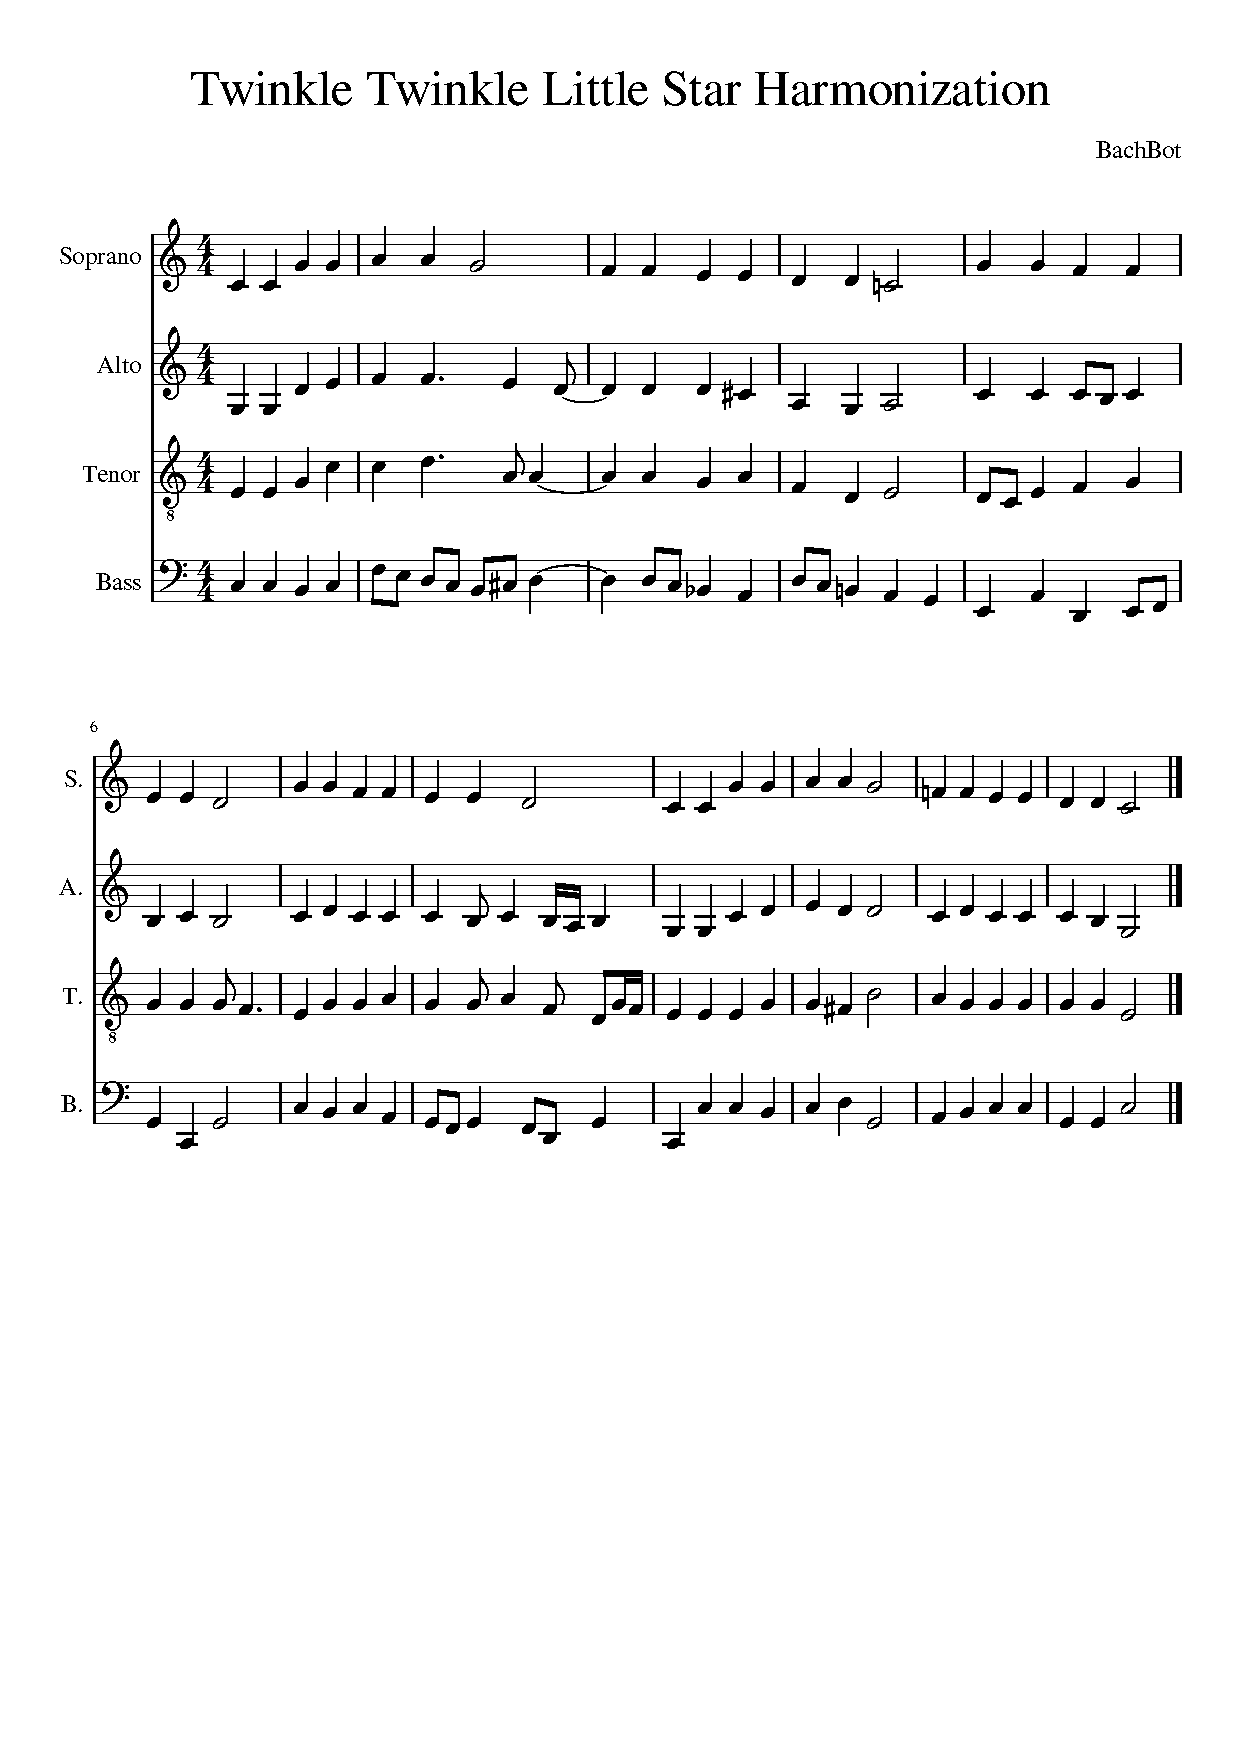
\includegraphics[trim={0 10cm 0 3.7cm},clip,width=0.9\linewidth]{twinkle-twinkle-score.pdf}
  \caption{BachBot's ATB harmonization to a \textit{Twinkle Twinkle Little Star} melody}
  \label{fig:harm-twinkle-twinkle}
\end{figure}

To our surprise, we found that BachBot was not only able to generate a
harmonically pleasant harmonization, but that \emph{the harmonization exhibited
features reminiscent of Bach's Baroque style}. This result demonstrates that
BachBot has successfully extracted statistical regularities from its input
corpus which are involved in giving Baroque music its sense of style.
